\documentclass{article}
\usepackage[utf8]{inputenc}
\usepackage[spanish]{babel}
\usepackage{listings}
\usepackage{subfigure}
\usepackage{graphicx}
\usepackage{url}
\usepackage{multirow}
\usepackage{color}
\usepackage{booktabs}
\usepackage{float}
\usepackage{amsmath}
\usepackage{hyperref}

\usepackage[margin=3cm,twoside]{geometry} 
\setlength{\parindent}{0pt}
\setlength{\parskip}{1em}


\definecolor{mygreen}{rgb}{0,0.6,0}
\definecolor{mygray}{rgb}{0.5,0.5,0.5}
\definecolor{mymauve}{rgb}{0.58,0,0.82}
\lstset{ 
  backgroundcolor=\color{white},   % choose the background color; you must add \usepackage{color} or \usepackage{xcolor}; should come as last argument
  basicstyle=\footnotesize,        % the size of the fonts that are used for the code
  breakatwhitespace=false,         % sets if automatic breaks should only happen at whitespace
  breaklines=true,                 % sets automatic line breaking
  captionpos=b,                    % sets the caption-position to bottom
  commentstyle=\color{mygreen},    % comment style
  deletekeywords={...},            % if you want to delete keywords from the given language
  escapeinside={\%*}{)},          % if you want to add LaTeX within your code
  extendedchars=true,              % lets you use non-ASCII characters; for 8-bits encodings only, does not work with UTF-8
  firstnumber=1,                % start line enumeration with line 1000
  frame=single,	                   % adds a frame around the code
  keepspaces=true,                 % keeps spaces in text, useful for keeping indentation of code (possibly needs columns=flexible)
  keywordstyle=\color{blue},       % keyword style
  language=Octave,                 % the language of the code
  morekeywords={*,...},            % if you want to add more keywords to the set
  numbers=left,                    % where to put the line-numbers; possible values are (none, left, right)
  numbersep=5pt,                   % how far the line-numbers are from the code
  numberstyle=\tiny\color{mygray}, % the style that is used for the line-numbers
  rulecolor=\color{black},         % if not set, the frame-color may be changed on line-breaks within not-black text (e.g. comments (green here))
  showspaces=false,                % show spaces everywhere adding particular underscores; it overrides 'showstringspaces'
  showstringspaces=false,          % underline spaces within strings only
  showtabs=false,                  % show tabs within strings adding particular underscores
  stepnumber=1,                    % the step between two line-numbers. If it's 1, each line will be numbered
  stringstyle=\color{mymauve},     % string literal style
  tabsize=2,	                   % sets default tabsize to 2 spaces
  title=\lstname                  % show the filename of files included with \lstinputlisting; also try caption instead of title
}
\usepackage{etoolbox}
\makeatletter
\providecommand{\subtitle}[1]{% add subtitle to \maketitle
  \apptocmd{\@title}{\par {\large #1 \par}}{}{}
}
\renewcommand{\theenumi}{\roman{enumi}}
\newtheorem{teor}{Teorema}
\makeatother
\title{Tarea 5 de Modelos Probabilistas Aplicados}
\subtitle{Algoritmos generadores de números pseudo-aleatorios con distribución Uniforme y distribución Normal}

\author{5271}
\date{\today}

\begin{document}

\maketitle

\section{Introducción}

En este trabajo se presenta el análisis a varios algoritmos de generación de números pseudo-aleatorios con distribución Uniforme y distribución Normal. Así como el impacto de los parámetros de dichos algoritmos en la calidad de los números pseudo-aleatorios. El análisis será realizado en el programa R versión 4.0.2 \cite{r} en el entorno de desarrollo Rstudio \cite{rstudio}

\section{Generador congruencial lineal(Mixto)}

Entre los principales generadores de números pseudo-aleatorios que se emplean en la actualidad están los llamados generadores congruenciales lineales, introducidos por Lehmer en 1951. Estos métodos comienza con un valor inicial $x_{0}$ (semilla), y los sucesivos valores $x_{n}, n\geq 0$ se obtienen recursivamente con la ecuación \ref{eq:1}:
\begin{equation}
    X_{n+1}= (aX_{n}+c)\: mod \: m,\quad n\geq 0.
    \label{eq:1}
\end{equation}
Con parámetros:
\begin{equation}\label{eq:2}
\begin{array}{llll}

 m, & el\:  m\acute{o}dulo;& 0<m.\\
 a, & el\:  multiplicador;& 0\leq a<m.\\
 c, & el\:  incremento;& 0\leq c<m.\\
 X_{0},& la\:  semilla;& 0\leq X_{0}<m.
\end{array}
\end{equation}

Se crea una función con la ecuación \ref{eq:1} en R, como muestra el código \ref{eq:1}. 
\begin{center}
\lstinputlisting[ language=R, firstline=1, lastline=12]{Tarea5.R}
\label{cod:1}
\end{center}

Pero con esto no es suficiente para garantizar la calidad de los números pseudos-aleatorios, una de estas medidas de calidad es el período de los números generados. El período no es más que cada cuentos números generados se vuelve a repetir la secuencia y se representa $\lambda^{*}(m)$ es decir que si $\lambda^{*}<m$ el generador no es de buena calidad. Los generadores de buena calidad deben tener un período completo, es decir $\lambda^{*}(m)=m$. Para garantizar el período completo se tiene de \cite{glc}:
\begin{teor}
La secuencia lineal congruencial definida por $m,\: a,\: c,\: X_{0}$ tiene período completo sí y solo sí
\begin{enumerate}
\item $c$ es primo relativo de $m$.
\item $b=a-1$ es múltiplo de $p, \forall\: p$ primo dividiendo $m$. 
\item $b$ es múltiplo de cuatro, sí $m$ es un múltiplo de cuatro.
\end{enumerate}
\end{teor}
\subsection{Selección del módulo}
Para la selección del modulo $m$ la siguiente expresión:
\begin{equation}
m = P^{e} \left\lbrace
\begin{array}{ll}
\textup{P}\: es \:la\: base \:que \:utiliza\\
\textup{}\\
\textup{e} \:es\: el\: n\acute{u}mero \:de \:bit
\end{array}
\right.
\end{equation}
La base mayormente usada es dos y el número de bit es 32.Para la selección del valor para el módulo se creo la función \ref{cod:2} en R.

\begin{center}
\lstinputlisting[ language=R, firstline=52, lastline=54]{Tarea5.R}
\label{cod:2}
\end{center}

\subsection{Selección del incremento}
El incremento o constante aditiva $c$ es un número en el intervalo $0\leq c<m$ y primo relativo con $m$, es decir que el Mínimo Común Divisor de $(c,m)= 1$, esto genera una cierta cantidad de posibles valores de $c$. Para garantizar la elección de un valor de $c$ adecuado se realizo una la función \ref{cod:3} en R. 

\begin{center}
\lstinputlisting[ language=R, firstline=35, lastline=44]{Tarea5.R}
\label{cod:3}
\end{center}

\subsection{Selección del multiplicador}
Para la elección acertada del multiplicador $a$ se tiene las siguientes expresiones:

$a=1+MCM(P_{1},P_{2},P_{3},...,P_{k-1,P_{k},4})*t, \quad t \in (Z^{+} \cup \left\{0 \right\} )$ si cuatro divide a $m$.

$a=1+MCM(P_{1},P_{2},P_{3},...,P_{k-1,P_{k}})*t, \quad t \in (Z^{+} \cup \left\{0 \right\} )$ si cuatro no divide a $m$.

Teniendo en cuenta estas expresiones y con el apoyo en la función \textit{LCM} de R que calcula el Mínimo Común Múltiplo (MCM), se crea la función \ref{cod:4} en R para la correcta selección del parámetro $a$.

\begin{center}
\lstinputlisting[ language=R, firstline=15, lastline=33]{Tarea5.R}
\label{cod:4}
\end{center}
\subsection{Selección de la semilla}
Para la selección de la semilla $X_{0}$ solo se debe tener en cuenta que debe encontrarse en el rango $0\leq X_{0}<m$.
\subsection{Generador congruencial lineal(Mixto) de período completo}

Con las funciones \ref{cod:2}, \ref{cod:3}, \ref{cod:4}, se modifica la función \ref{cod:1}, dando lugar a la función \ref{cod:5} que garantiza el período completo y la posibilidad de reproducir la secuencia si fuera necesario, dando como resultados números pseudo-aleatorios de calidad. Esto se comprueba en la figura \ref{fig:1} de la página \pageref{fig:1} y en los resultados de la prueba estadística de uniformidad e independencia Chi-cuadrado con un valor del estadístico $X^{2}=11.424$ y el valor p = $0.9088$, no se rechaza la hipótesis nula. Por tanto, los números son independientes y uniformes. 
\begin{center}
\lstinputlisting[ language=R, firstline=57, lastline=69]{Tarea5.R}
\label{cod:5}
\end{center}
\begin{figure}
\centering
\subfigure[Histogramas de frecuencia de los números pseudo-aleatorios creados por la función \textit{uniformeGCL} presentada y \textit{runif} de R. ]{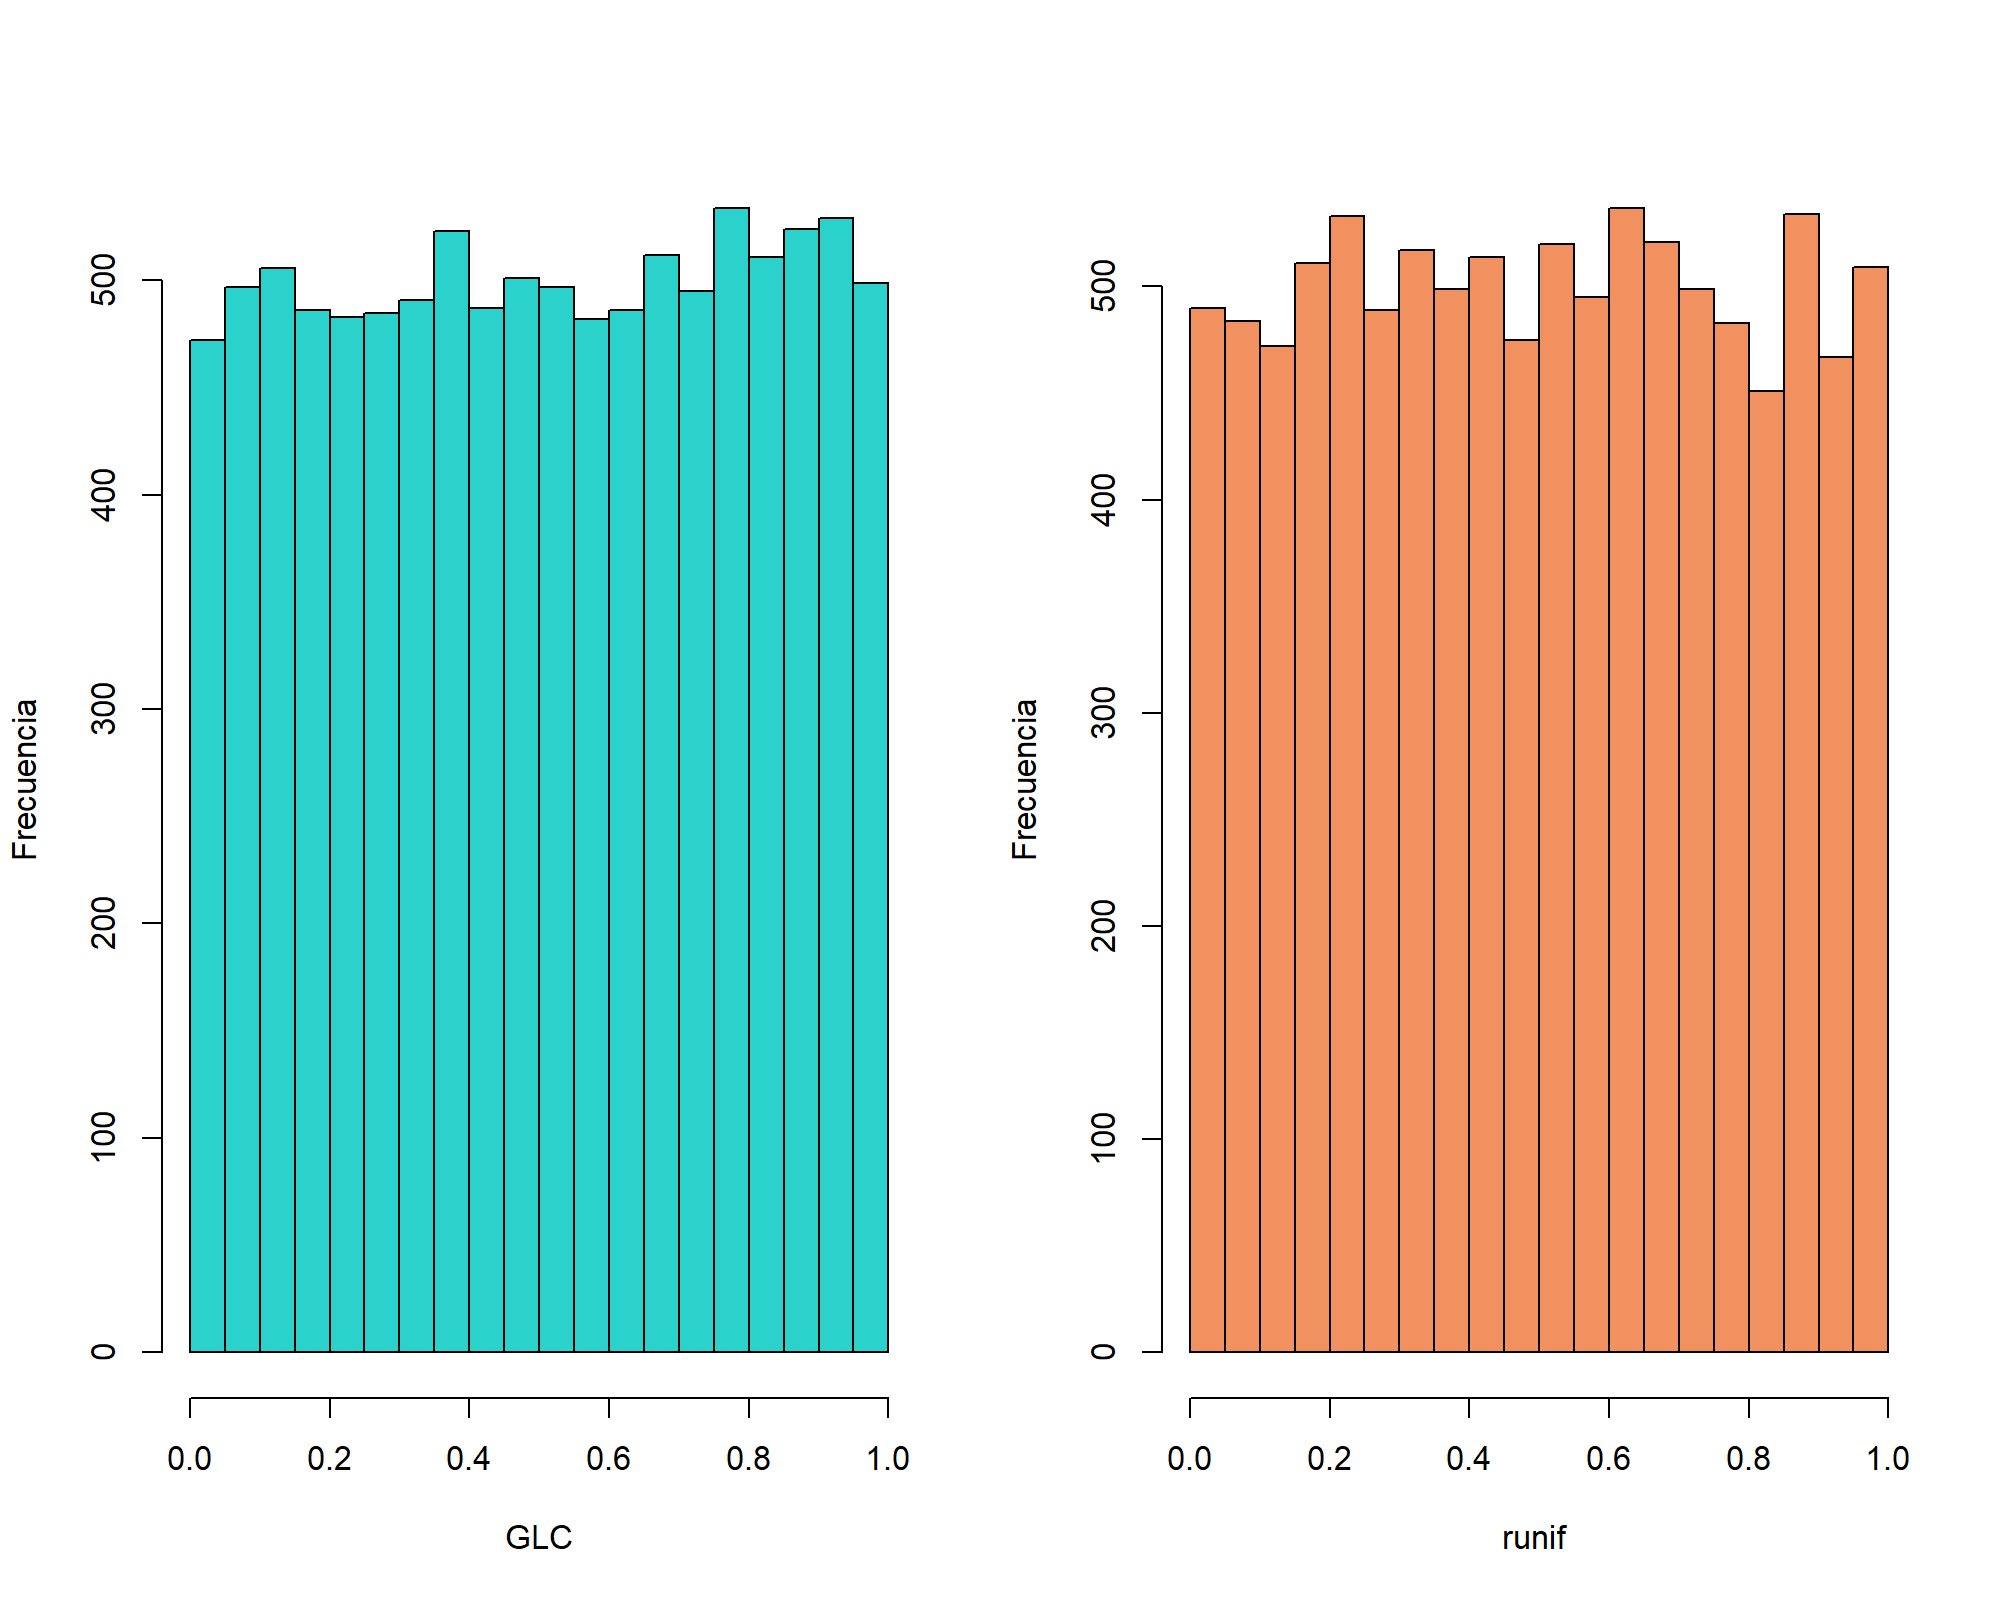
\includegraphics[scale=0.50]{figuras/AproxGU10000.png}}
\vspace{-0.3cm}
\centering
\subfigure[Diagrama de densidad de ambas poblaciones generadas decreciente]{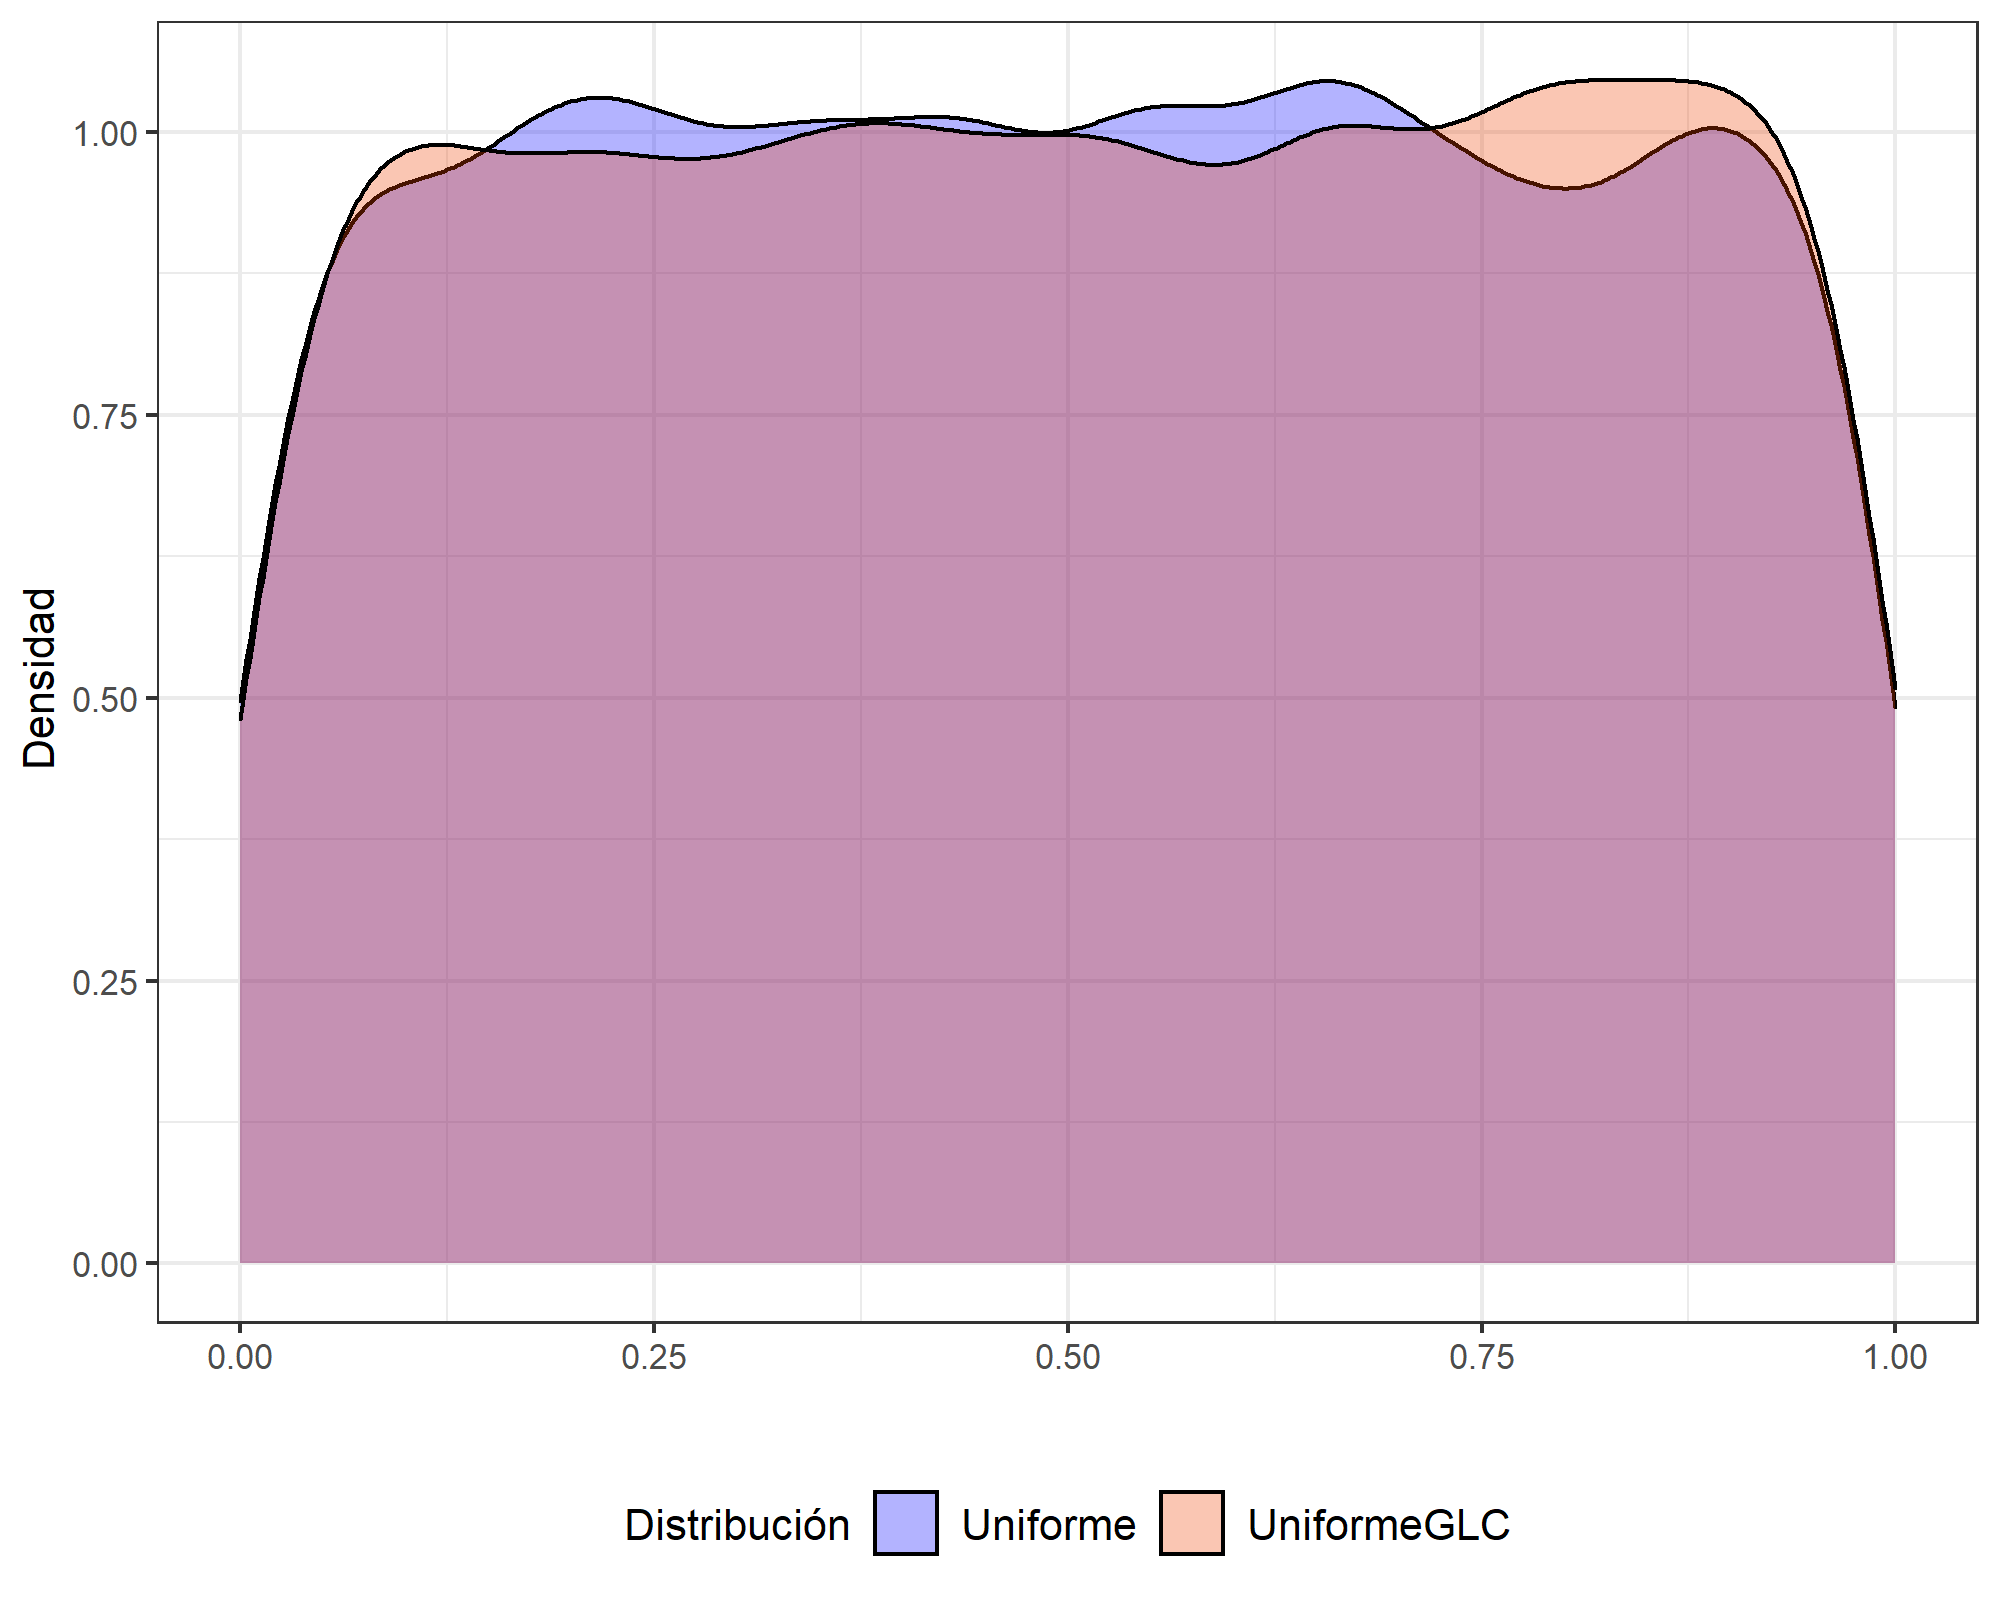
\includegraphics[scale=0.50]{figuras/densidadUG.png}}
\caption{Comparación de ambos métodos de generación de números pseudo-aleatorios}
\label{fig:1} 
\end{figure}
\section{Transformada de Box-Muller}
la Transformada de Box-Muller es  método para generar pares de independiente, estándar, normalmente distribuido. Este método fue llevado  a un programa de R como se muestra en el código \ref{cod:6}. A partir de este código se realizo una experimentación donde se variaron los parámetros $z_{0}$, $z_{1}$ y se utilizó en uno de los casos el generador \textit{uniformeGLC} propuesto. 

\begin{center}
\lstinputlisting[ language=R, firstline=79, lastline=84]{Tarea5.R}
\label{cod:6}
\end{center}

En la imagen \ref{fig:2} de la página \pageref{fig:2}  se muestran los histogramas de las diferentes variantes analizadas, como se puede observar la variante la sdos variantes representan una distribución normal, por la prueba de Shapiro–Wilk con un valor p de 0.98 para la a) y 0.87 para b). 
\begin{figure}

\centering
\subfigure[Histograma de frecuencia de la distribución normal creada por \textit{runif} ]{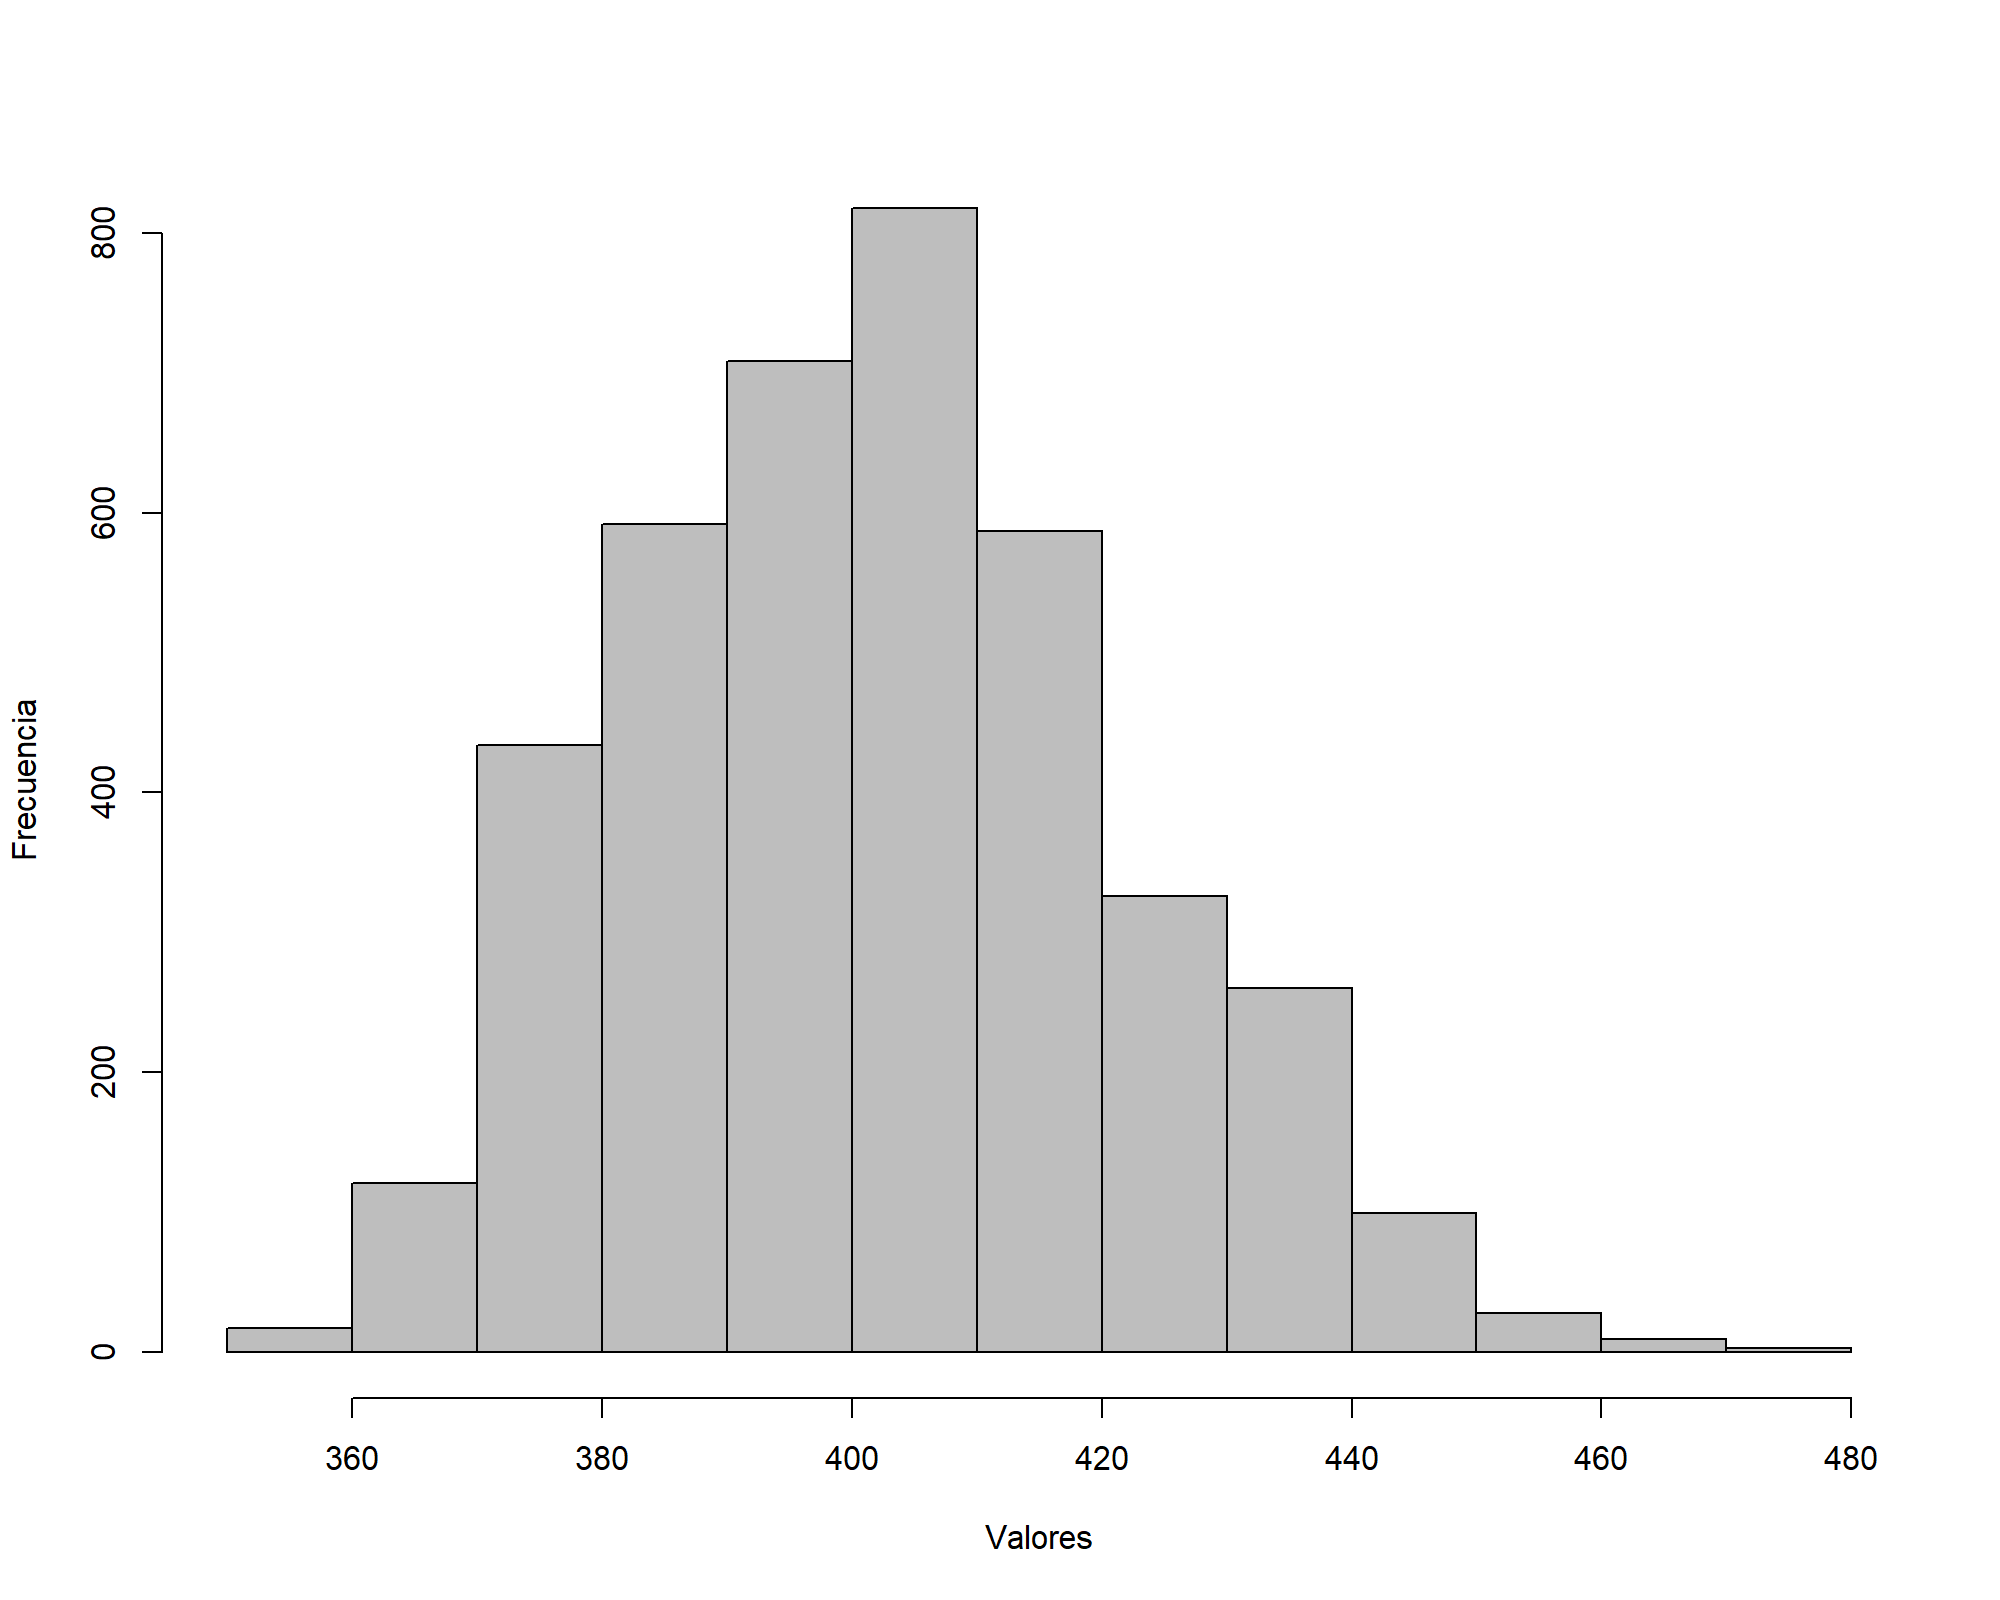
\includegraphics[scale=0.50]{figuras/4.png}}
\vspace{-0.3cm}
\centering
\subfigure[Histograma de frecuencia de la distribución normal creada por \textit{UniformeGLC} ]{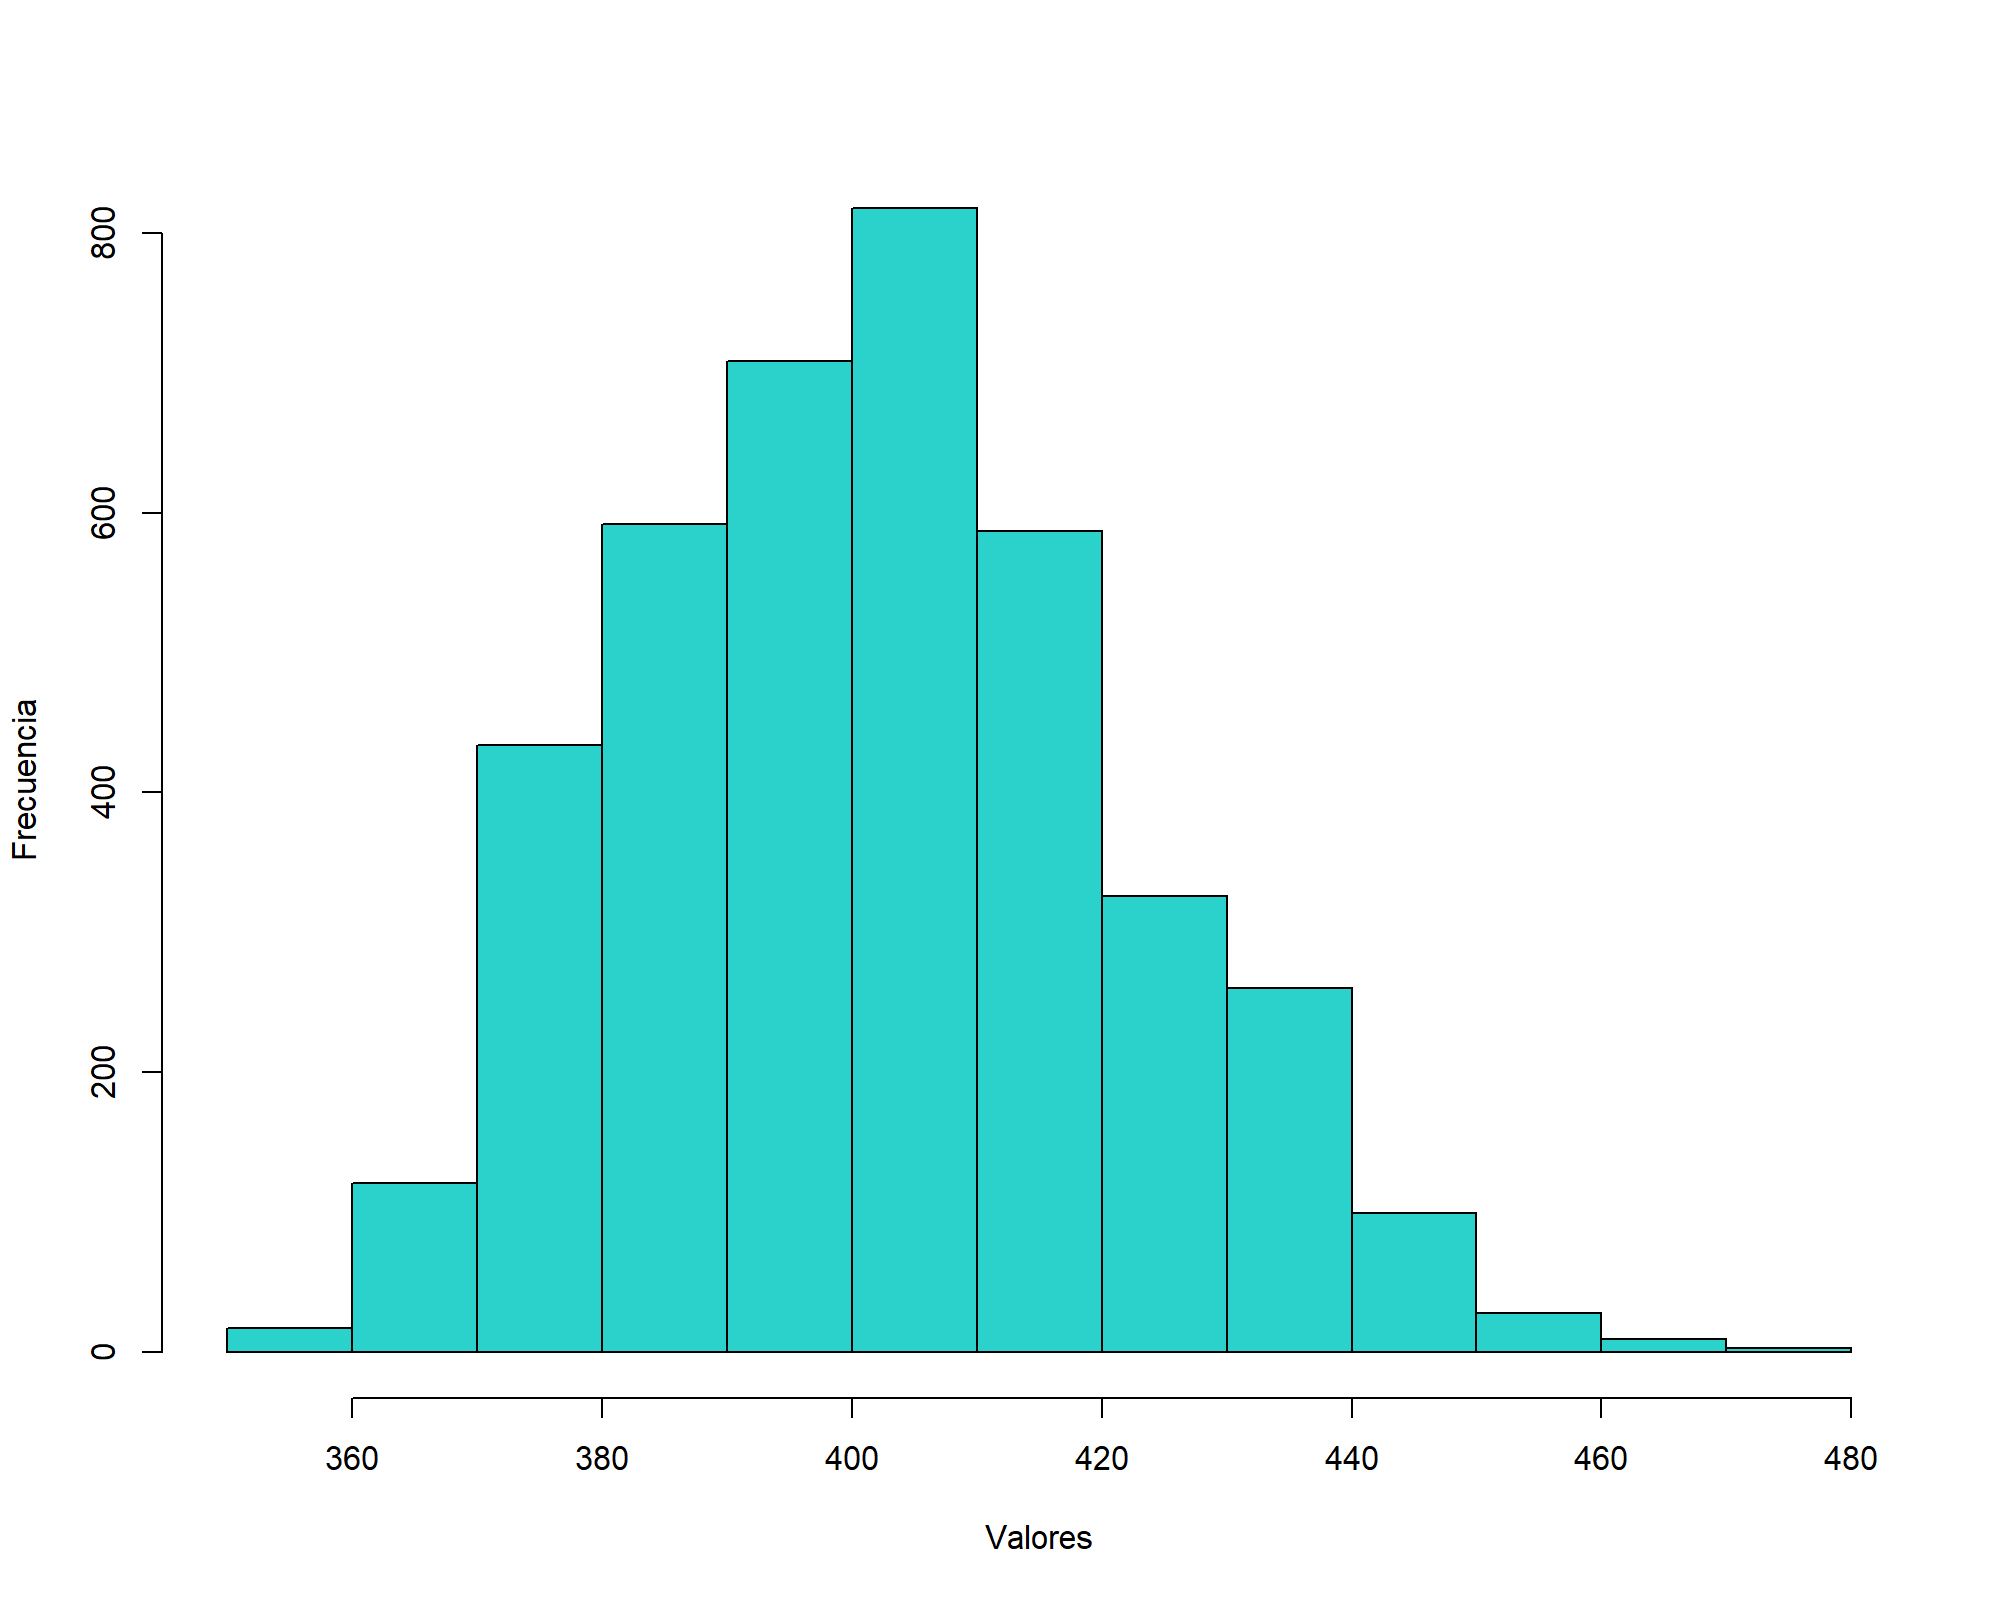
\includegraphics[scale=0.50]{figuras/5.png}}
\caption{Comparación de ambos métodos de generación de números pseudo-aleatorios}
\label{fig:2} 
\end{figure}

El código general se encuentra disponible en el repositorio. \href{https://github.com/Albertomnoa/Tareas_MPA/tree/master/Tarea4}{https://github.com/Albertomnoa/Tareas} 

\newpage
\bibliographystyle{plain}
\bibliography{Biblio}

\end{document}
